\documentclass[a4paper,12pt]{report}
%\documentclass[a4paper,10pt]{scrartcl}

\usepackage{gfsneohellenic}
\usepackage{xltxtra}
\usepackage{pdfpages}
\usepackage{xcolor}
\usepackage{fancybox, graphicx}
\usepackage{xgreek} % Greek hyphenation
\usepackage[scale=0.77]{geometry}
\usepackage{array}
\usepackage{multirow}

\setromanfont[Mapping=tex-text]{GFS Neohellenic}
\setsansfont[Mapping=tex-text]{GFS Neohellenic}
\setmonofont[Mapping=tex-text]{GFS Neohellenic}

\newcounter{nextyear}
\renewcommand{\thesection}{\Roman{section}}
\makeatletter
\renewcommand\part{%
  \if@openright
    \cleardoublepage
  \else
    \clearpage
  \fi
  \thispagestyle{empty}%   % Original »plain« replaced by »emptyx
  \if@twocolumn
    \onecolumn
    \@tempswatrue
  \else
    \@tempswafalse
  \fi
  \null\vfil
  \secdef\@part\@spart}
\makeatother

\title{
\vspace{-2.5cm}
\line(1,0){440}\\
\vspace{0.5cm}
Φοιτητικός Σύλλογος Πληροφορικής και Τηλεματικής\\
\vspace{0.3cm}
\line(1,0){440}\\
\vspace{0.7cm} 
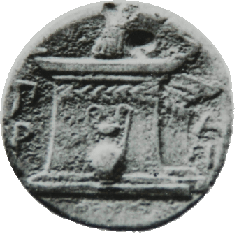
\includegraphics[scale=0.22]{hua.png} \\
\line(1,0){400}\\
\vspace{0.5cm}
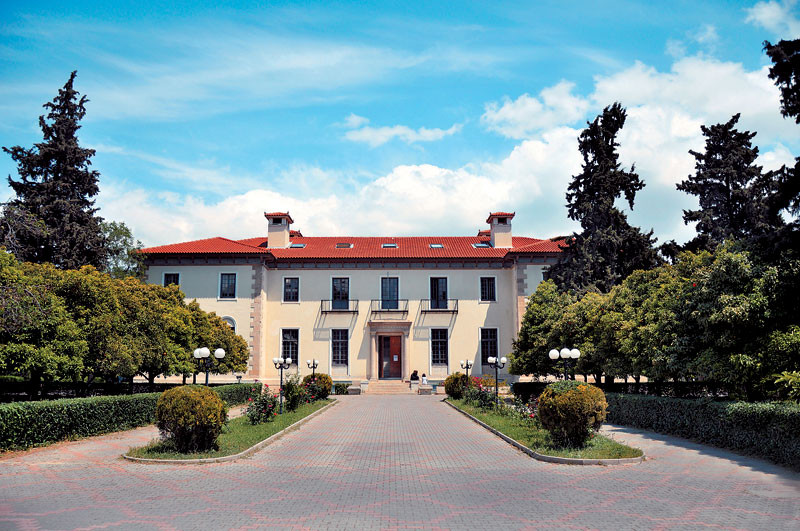
\includegraphics[scale=0.495]{xarokopeio.jpg}
\vspace{0.5cm}
\line(1,0){400}\\
}
\author{}
\date{
\vspace{0.2cm}
Έτος \the\year \space- \thenextyear
}

\begin{document}
\color{blue!20!black!95}
\setcounter{nextyear}{\year}
\addtocounter{nextyear}{1}
\centering
\doublebox{
\begin{minipage}{\hsize}\
\centering
\maketitle
\end{minipage}
}

\Roman{part}
\Roman{section}

\part{Ο Σύλλογος}
\pagenumbering{Roman}
\section[Αποτελέσματα]{Τα Αποτελέσματα της ψηφοφορίας για το έτος \the\year \space- \thenextyear \space είναι :}
\vspace{0.5cm}
\begin{large}
\begin{center}
\begin{tabular}{|>{\centering\arraybackslash}p{1cm} | >{\centering\arraybackslash}p{8cm} | >{\centering\arraybackslash}p{1.5cm}|}
  \hline
  \multicolumn{1}{|c}{Θέση} & \multicolumn{1}{c}{Ονοματεπώνυμο} & \multicolumn{1}{c|}{Ψήφοι}\\
  \hline
  1 & Παναγιώτης Ευστρατιάδης & \\ \hline
  2 & Ανδρέας Γρίβας & \\ \hline
  3 & Βασιλεία Παπαιωάννου & \\ \hline
  4 & Χριστίνα Μπαμπασανίδη & \\ \hline
  5 & Ξενοφών Δρίτσουλας & \\ \hline
  6 & - & \\ \hline
  7 & - & \\ \hline
  8 & - & \\ \hline
  9 & - & \\ \hline
  10 & - & \\ \hline
  11 & - & \\ \hline
  12 & - & \\ \hline
  13 & - & \\ \hline
  14 & - & \\ \hline
  15 & - & \\ \hline
  16 & - & \\ \hline
  17 & - & \\ \hline
  18 & - & \\ \hline
  19 & - & \\ \hline
  20 & - & \\ \hline
  21 & - & \\ \hline
  22 & - & \\ \hline
  23 & - & \\ \hline
  24 & - & \\ \hline
  25 & - & \\ \hline
  \multicolumn{2}{|c|}{Άκυρα} & \multicolumn{1}{c|}{} \\ \hline
  \multicolumn{2}{|c|}{Λευκά} & \multicolumn{1}{c|}{} \\ \hline
  \multicolumn{2}{|c|}{Σύνολο} & \multicolumn{1}{c|}{} \\ \hline
\end{tabular}
\vspace{0.5cm}
\end{center}
\end{large}
\large{Απο τα πάνω στοιχεία φαίνεται πως απαρτία σχηματίζεται με \line(1,0){40} \hspace{0.15cm} φοιτητές.}

\newpage
\section[Μέλη ΔΣ]{Τα Μέλη του ΔΣ το έτος \the\year \space- \thenextyear \space είναι :}
\vspace{1cm}

\begin{Large}
\begin{center}
\begin{tabular}{|l|c|}
  \hline
  \multicolumn{1}{|c}{Θέση} & \multicolumn{1}{c|}{Ονοματεπώνυμο} \\
  \hline
  Πρόεδρος & Παναγιώτης Ευστρατιάδης \\ \hline
  Αντιπρόεδρος & Ανδρέας Γρίβας \\ \hline
  Ταμίας & Βασιλεία Παπαιωάννου \\ \hline
  Γενικός Γραμματέας & Χριστίνα Μπαμπασανίδη \\ \hline
  Ειδικός Γραμματέας & Ξενοφών Δρίτσουλας \\ \hline
  Μέλος Α' & - \\ \hline
  Μέλος Β' & - \\ \hline
\end{tabular}
\vspace{0.5cm}
\end{center}
\end{Large}

\begin{large}
\paragraph{}
Ως Φοιτητικός Σύλλογος Πληροφορικής και Τηλεματικής δηλώνουμε υπεύθυνα πως έχουμε διαβάσει το καταστατικό λειτουργίας
του συλλόγου και δεσμευόμαστε να το τηρούμε και να το υπερασπίσουμε μέχρι το τέλος της θήτειας μας ή μέχρις ότου αλλάξει η διαδικασία ή το καταστατικό
μετά από απόφαση γενικής συνέλευσης.
\vspace{0.5cm}

\begin{center}
\begin{tabular}{>{\centering\arraybackslash}p{4.5cm} c >{\centering\arraybackslash}p{4.5cm} c >{\centering\arraybackslash}p{4.5cm}}
\centering
Ο Πρόεδρος && Ο Αντιπρόεδρος && Ο Ταμίας \\
&&&& \\
&&&& \\
\cline{1-1}  \cline{3-3}  \cline{5-5} \\
\end{tabular}
\end{center}

\vspace{0.5cm}

\begin{center}
\begin{tabular}{>{\centering\arraybackslash}p{4.5cm} c >{\centering\arraybackslash}p{4.5cm}}
\centering
Ο Γ.Γραμματέας && Ο Ε.Γραμματέας\\
&& \\
&& \\
\cline{1-1}  \cline{3-3}\\
\end{tabular}
\end{center}

\vspace{0.5cm}

\begin{center}
\begin{tabular}{>{\centering\arraybackslash}p{4.5cm} c >{\centering\arraybackslash}p{4.5cm}}
\centering
&Τα Μέλη&\\
&& \\
&& \\
\cline{1-1}  \cline{3-3}\\
\end{tabular}
\end{center}
\end{large}



\part{Τα Πρακτικά}
\pagenumbering{arabic}
\setcounter{section}{0}
\section{Συνεδρίαση ΔΣ}
\begin{Large}
\begin{tabular}{|l|>{\centering\arraybackslash}p{5.2cm}|}
\hline
Ημερομηνία & { \hspace{0.7cm}-\hspace{0.7cm}-\hspace{1.4cm}} \\ \hline
\end{tabular}
\end{Large}
\vspace{1cm}
\section{Συζητήθηκαν}
\begin{Large}
\begin{enumerate}
 \item \line(1,0){425} \\
 \line(1,0){425} \\
 \line(1,0){425} \\
 \item \line(1,0){425} \\
 \line(1,0){425} \\
 \line(1,0){425} \\
  \item \line(1,0){425} \\
 \line(1,0){425} \\
 \line(1,0){425} \\
  \item \line(1,0){425} \\
 \line(1,0){425} \\
 \line(1,0){425} \\
  \item \line(1,0){425} \\
 \line(1,0){425} \\
 \line(1,0){425} \\

\end{enumerate}
\begin{center}
\line(1,0){440} \\
\line(1,0){440} \\
\line(1,0){440} \\
\line(1,0){440} \\
\line(1,0){440} \\
\end{center}
\end{Large}
\newpage
\section{Προτάθηκαν για θέματα Γενικής Συνέλευσης}
\vspace{1cm}
\begin{Large}
\begin{enumerate}
 \item \line(1,0){425} \\
 \line(1,0){425} \\
 \item \line(1,0){425} \\
 \line(1,0){425} \\
  \item \line(1,0){425} \\
 \line(1,0){425} \\
  \item \line(1,0){425} \\
 \line(1,0){425} \\
  \item \line(1,0){425} \\
 \line(1,0){425} \\

\end{enumerate}
\begin{center}
\line(1,0){440} \\
\line(1,0){440} \\
\line(1,0){440} \\
\line(1,0){440} \\
\line(1,0){440} \\
\end{center}
\end{Large}


\vspace{1cm}
\begin{center}
\begin{tabular}{>{\centering\arraybackslash}p{4.5cm} c >{\centering\arraybackslash}p{4.5cm} c >{\centering\arraybackslash}p{4.5cm}}
\centering
Ο Πρόεδρος && Ο Αντιπρόεδρος && Ο Ταμίας \\
&&&& \\
&&&& \\
\cline{1-1}  \cline{3-3}  \cline{5-5} \\
\end{tabular}
\end{center}

\vspace{0.5cm}

\begin{center}
\begin{tabular}{>{\centering\arraybackslash}p{4.5cm} c >{\centering\arraybackslash}p{4.5cm}}
\centering
Ο Γ.Γραμματέας && Ο Ε.Γραμματέας\\
&& \\
&& \\
\cline{1-1}  \cline{3-3}\\
\end{tabular}
\end{center}

\vspace{0.5cm}
\newpage
\setcounter{section}{0}
\section{Συνεδρίαση ΔΣ}
\begin{Large}
\begin{tabular}{|l|>{\centering\arraybackslash}p{5.2cm}|}
\hline
Ημερομηνία & { \hspace{0.7cm}-\hspace{0.7cm}-\hspace{1.4cm}} \\ \hline
\end{tabular}
\end{Large}
\vspace{1cm}
\section{Συζητήθηκαν}
\begin{Large}
\begin{enumerate}
 \item \line(1,0){425} \\
 \line(1,0){425} \\
 \line(1,0){425} \\
 \item \line(1,0){425} \\
 \line(1,0){425} \\
 \line(1,0){425} \\
  \item \line(1,0){425} \\
 \line(1,0){425} \\
 \line(1,0){425} \\
  \item \line(1,0){425} \\
 \line(1,0){425} \\
 \line(1,0){425} \\
  \item \line(1,0){425} \\
 \line(1,0){425} \\
 \line(1,0){425} \\

\end{enumerate}
\begin{center}
\line(1,0){440} \\
\line(1,0){440} \\
\line(1,0){440} \\
\line(1,0){440} \\
\line(1,0){440} \\
\end{center}
\end{Large}
\newpage
\section{Προτάθηκαν για θέματα Γενικής Συνέλευσης}
\vspace{1cm}
\begin{Large}
\begin{enumerate}
 \item \line(1,0){425} \\
 \line(1,0){425} \\
 \item \line(1,0){425} \\
 \line(1,0){425} \\
  \item \line(1,0){425} \\
 \line(1,0){425} \\
  \item \line(1,0){425} \\
 \line(1,0){425} \\
  \item \line(1,0){425} \\
 \line(1,0){425} \\

\end{enumerate}
\begin{center}
\line(1,0){440} \\
\line(1,0){440} \\
\line(1,0){440} \\
\line(1,0){440} \\
\line(1,0){440} \\
\end{center}
\end{Large}


\vspace{1cm}
\begin{center}
\begin{tabular}{>{\centering\arraybackslash}p{4.5cm} c >{\centering\arraybackslash}p{4.5cm} c >{\centering\arraybackslash}p{4.5cm}}
\centering
Ο Πρόεδρος && Ο Αντιπρόεδρος && Ο Ταμίας \\
&&&& \\
&&&& \\
\cline{1-1}  \cline{3-3}  \cline{5-5} \\
\end{tabular}
\end{center}

\vspace{0.5cm}

\begin{center}
\begin{tabular}{>{\centering\arraybackslash}p{4.5cm} c >{\centering\arraybackslash}p{4.5cm}}
\centering
Ο Γ.Γραμματέας && Ο Ε.Γραμματέας\\
&& \\
&& \\
\cline{1-1}  \cline{3-3}\\
\end{tabular}
\end{center}

\vspace{0.5cm}
\newpage
\setcounter{section}{0}
\section{Συνεδρίαση ΔΣ}
\begin{Large}
\begin{tabular}{|l|>{\centering\arraybackslash}p{5.2cm}|}
\hline
Ημερομηνία & { \hspace{0.7cm}-\hspace{0.7cm}-\hspace{1.4cm}} \\ \hline
\end{tabular}
\end{Large}
\vspace{1cm}
\section{Συζητήθηκαν}
\begin{Large}
\begin{enumerate}
 \item \line(1,0){425} \\
 \line(1,0){425} \\
 \line(1,0){425} \\
 \item \line(1,0){425} \\
 \line(1,0){425} \\
 \line(1,0){425} \\
  \item \line(1,0){425} \\
 \line(1,0){425} \\
 \line(1,0){425} \\
  \item \line(1,0){425} \\
 \line(1,0){425} \\
 \line(1,0){425} \\
  \item \line(1,0){425} \\
 \line(1,0){425} \\
 \line(1,0){425} \\

\end{enumerate}
\begin{center}
\line(1,0){440} \\
\line(1,0){440} \\
\line(1,0){440} \\
\line(1,0){440} \\
\line(1,0){440} \\
\end{center}
\end{Large}
\newpage
\section{Προτάθηκαν για θέματα Γενικής Συνέλευσης}
\vspace{1cm}
\begin{Large}
\begin{enumerate}
 \item \line(1,0){425} \\
 \line(1,0){425} \\
 \item \line(1,0){425} \\
 \line(1,0){425} \\
  \item \line(1,0){425} \\
 \line(1,0){425} \\
  \item \line(1,0){425} \\
 \line(1,0){425} \\
  \item \line(1,0){425} \\
 \line(1,0){425} \\

\end{enumerate}
\begin{center}
\line(1,0){440} \\
\line(1,0){440} \\
\line(1,0){440} \\
\line(1,0){440} \\
\line(1,0){440} \\
\end{center}
\end{Large}


\vspace{1cm}
\begin{center}
\begin{tabular}{>{\centering\arraybackslash}p{4.5cm} c >{\centering\arraybackslash}p{4.5cm} c >{\centering\arraybackslash}p{4.5cm}}
\centering
Ο Πρόεδρος && Ο Αντιπρόεδρος && Ο Ταμίας \\
&&&& \\
&&&& \\
\cline{1-1}  \cline{3-3}  \cline{5-5} \\
\end{tabular}
\end{center}

\vspace{0.5cm}

\begin{center}
\begin{tabular}{>{\centering\arraybackslash}p{4.5cm} c >{\centering\arraybackslash}p{4.5cm}}
\centering
Ο Γ.Γραμματέας && Ο Ε.Γραμματέας\\
&& \\
&& \\
\cline{1-1}  \cline{3-3}\\
\end{tabular}
\end{center}

\vspace{0.5cm}
\newpage
\setcounter{section}{0}
\section{Συνεδρίαση ΔΣ}
\begin{Large}
\begin{tabular}{|l|>{\centering\arraybackslash}p{5.2cm}|}
\hline
Ημερομηνία & { \hspace{0.7cm}-\hspace{0.7cm}-\hspace{1.4cm}} \\ \hline
\end{tabular}
\end{Large}
\vspace{1cm}
\section{Συζητήθηκαν}
\begin{Large}
\begin{enumerate}
 \item \line(1,0){425} \\
 \line(1,0){425} \\
 \line(1,0){425} \\
 \item \line(1,0){425} \\
 \line(1,0){425} \\
 \line(1,0){425} \\
  \item \line(1,0){425} \\
 \line(1,0){425} \\
 \line(1,0){425} \\
  \item \line(1,0){425} \\
 \line(1,0){425} \\
 \line(1,0){425} \\
  \item \line(1,0){425} \\
 \line(1,0){425} \\
 \line(1,0){425} \\

\end{enumerate}
\begin{center}
\line(1,0){440} \\
\line(1,0){440} \\
\line(1,0){440} \\
\line(1,0){440} \\
\line(1,0){440} \\
\end{center}
\end{Large}
\newpage
\section{Προτάθηκαν για θέματα Γενικής Συνέλευσης}
\vspace{1cm}
\begin{Large}
\begin{enumerate}
 \item \line(1,0){425} \\
 \line(1,0){425} \\
 \item \line(1,0){425} \\
 \line(1,0){425} \\
  \item \line(1,0){425} \\
 \line(1,0){425} \\
  \item \line(1,0){425} \\
 \line(1,0){425} \\
  \item \line(1,0){425} \\
 \line(1,0){425} \\

\end{enumerate}
\begin{center}
\line(1,0){440} \\
\line(1,0){440} \\
\line(1,0){440} \\
\line(1,0){440} \\
\line(1,0){440} \\
\end{center}
\end{Large}


\vspace{1cm}
\begin{center}
\begin{tabular}{>{\centering\arraybackslash}p{4.5cm} c >{\centering\arraybackslash}p{4.5cm} c >{\centering\arraybackslash}p{4.5cm}}
\centering
Ο Πρόεδρος && Ο Αντιπρόεδρος && Ο Ταμίας \\
&&&& \\
&&&& \\
\cline{1-1}  \cline{3-3}  \cline{5-5} \\
\end{tabular}
\end{center}

\vspace{0.5cm}

\begin{center}
\begin{tabular}{>{\centering\arraybackslash}p{4.5cm} c >{\centering\arraybackslash}p{4.5cm}}
\centering
Ο Γ.Γραμματέας && Ο Ε.Γραμματέας\\
&& \\
&& \\
\cline{1-1}  \cline{3-3}\\
\end{tabular}
\end{center}

\vspace{0.5cm}
\newpage
\setcounter{section}{0}
\section{Συνεδρίαση ΔΣ}
\begin{Large}
\begin{tabular}{|l|>{\centering\arraybackslash}p{5.2cm}|}
\hline
Ημερομηνία & { \hspace{0.7cm}-\hspace{0.7cm}-\hspace{1.4cm}} \\ \hline
\end{tabular}
\end{Large}
\vspace{1cm}
\section{Συζητήθηκαν}
\begin{Large}
\begin{enumerate}
 \item \line(1,0){425} \\
 \line(1,0){425} \\
 \line(1,0){425} \\
 \item \line(1,0){425} \\
 \line(1,0){425} \\
 \line(1,0){425} \\
  \item \line(1,0){425} \\
 \line(1,0){425} \\
 \line(1,0){425} \\
  \item \line(1,0){425} \\
 \line(1,0){425} \\
 \line(1,0){425} \\
  \item \line(1,0){425} \\
 \line(1,0){425} \\
 \line(1,0){425} \\

\end{enumerate}
\begin{center}
\line(1,0){440} \\
\line(1,0){440} \\
\line(1,0){440} \\
\line(1,0){440} \\
\line(1,0){440} \\
\end{center}
\end{Large}
\newpage
\section{Προτάθηκαν για θέματα Γενικής Συνέλευσης}
\vspace{1cm}
\begin{Large}
\begin{enumerate}
 \item \line(1,0){425} \\
 \line(1,0){425} \\
 \item \line(1,0){425} \\
 \line(1,0){425} \\
  \item \line(1,0){425} \\
 \line(1,0){425} \\
  \item \line(1,0){425} \\
 \line(1,0){425} \\
  \item \line(1,0){425} \\
 \line(1,0){425} \\

\end{enumerate}
\begin{center}
\line(1,0){440} \\
\line(1,0){440} \\
\line(1,0){440} \\
\line(1,0){440} \\
\line(1,0){440} \\
\end{center}
\end{Large}


\vspace{1cm}
\begin{center}
\begin{tabular}{>{\centering\arraybackslash}p{4.5cm} c >{\centering\arraybackslash}p{4.5cm} c >{\centering\arraybackslash}p{4.5cm}}
\centering
Ο Πρόεδρος && Ο Αντιπρόεδρος && Ο Ταμίας \\
&&&& \\
&&&& \\
\cline{1-1}  \cline{3-3}  \cline{5-5} \\
\end{tabular}
\end{center}

\vspace{0.5cm}

\begin{center}
\begin{tabular}{>{\centering\arraybackslash}p{4.5cm} c >{\centering\arraybackslash}p{4.5cm}}
\centering
Ο Γ.Γραμματέας && Ο Ε.Γραμματέας\\
&& \\
&& \\
\cline{1-1}  \cline{3-3}\\
\end{tabular}
\end{center}

\vspace{0.5cm}
\newpage
\setcounter{section}{0}
\section{Συνεδρίαση ΔΣ}
\begin{Large}
\begin{tabular}{|l|>{\centering\arraybackslash}p{5.2cm}|}
\hline
Ημερομηνία & { \hspace{0.7cm}-\hspace{0.7cm}-\hspace{1.4cm}} \\ \hline
\end{tabular}
\end{Large}
\vspace{1cm}
\section{Συζητήθηκαν}
\begin{Large}
\begin{enumerate}
 \item \line(1,0){425} \\
 \line(1,0){425} \\
 \line(1,0){425} \\
 \item \line(1,0){425} \\
 \line(1,0){425} \\
 \line(1,0){425} \\
  \item \line(1,0){425} \\
 \line(1,0){425} \\
 \line(1,0){425} \\
  \item \line(1,0){425} \\
 \line(1,0){425} \\
 \line(1,0){425} \\
  \item \line(1,0){425} \\
 \line(1,0){425} \\
 \line(1,0){425} \\

\end{enumerate}
\begin{center}
\line(1,0){440} \\
\line(1,0){440} \\
\line(1,0){440} \\
\line(1,0){440} \\
\line(1,0){440} \\
\end{center}
\end{Large}
\newpage
\section{Προτάθηκαν για θέματα Γενικής Συνέλευσης}
\vspace{1cm}
\begin{Large}
\begin{enumerate}
 \item \line(1,0){425} \\
 \line(1,0){425} \\
 \item \line(1,0){425} \\
 \line(1,0){425} \\
  \item \line(1,0){425} \\
 \line(1,0){425} \\
  \item \line(1,0){425} \\
 \line(1,0){425} \\
  \item \line(1,0){425} \\
 \line(1,0){425} \\

\end{enumerate}
\begin{center}
\line(1,0){440} \\
\line(1,0){440} \\
\line(1,0){440} \\
\line(1,0){440} \\
\line(1,0){440} \\
\end{center}
\end{Large}


\vspace{1cm}
\begin{center}
\begin{tabular}{>{\centering\arraybackslash}p{4.5cm} c >{\centering\arraybackslash}p{4.5cm} c >{\centering\arraybackslash}p{4.5cm}}
\centering
Ο Πρόεδρος && Ο Αντιπρόεδρος && Ο Ταμίας \\
&&&& \\
&&&& \\
\cline{1-1}  \cline{3-3}  \cline{5-5} \\
\end{tabular}
\end{center}

\vspace{0.5cm}

\begin{center}
\begin{tabular}{>{\centering\arraybackslash}p{4.5cm} c >{\centering\arraybackslash}p{4.5cm}}
\centering
Ο Γ.Γραμματέας && Ο Ε.Γραμματέας\\
&& \\
&& \\
\cline{1-1}  \cline{3-3}\\
\end{tabular}
\end{center}

\vspace{0.5cm}
\newpage
\setcounter{section}{0}
\section{Συνεδρίαση ΔΣ}
\begin{Large}
\begin{tabular}{|l|>{\centering\arraybackslash}p{5.2cm}|}
\hline
Ημερομηνία & { \hspace{0.7cm}-\hspace{0.7cm}-\hspace{1.4cm}} \\ \hline
\end{tabular}
\end{Large}
\vspace{1cm}
\section{Συζητήθηκαν}
\begin{Large}
\begin{enumerate}
 \item \line(1,0){425} \\
 \line(1,0){425} \\
 \line(1,0){425} \\
 \item \line(1,0){425} \\
 \line(1,0){425} \\
 \line(1,0){425} \\
  \item \line(1,0){425} \\
 \line(1,0){425} \\
 \line(1,0){425} \\
  \item \line(1,0){425} \\
 \line(1,0){425} \\
 \line(1,0){425} \\
  \item \line(1,0){425} \\
 \line(1,0){425} \\
 \line(1,0){425} \\

\end{enumerate}
\begin{center}
\line(1,0){440} \\
\line(1,0){440} \\
\line(1,0){440} \\
\line(1,0){440} \\
\line(1,0){440} \\
\end{center}
\end{Large}
\newpage
\section{Προτάθηκαν για θέματα Γενικής Συνέλευσης}
\vspace{1cm}
\begin{Large}
\begin{enumerate}
 \item \line(1,0){425} \\
 \line(1,0){425} \\
 \item \line(1,0){425} \\
 \line(1,0){425} \\
  \item \line(1,0){425} \\
 \line(1,0){425} \\
  \item \line(1,0){425} \\
 \line(1,0){425} \\
  \item \line(1,0){425} \\
 \line(1,0){425} \\

\end{enumerate}
\begin{center}
\line(1,0){440} \\
\line(1,0){440} \\
\line(1,0){440} \\
\line(1,0){440} \\
\line(1,0){440} \\
\end{center}
\end{Large}


\vspace{1cm}
\begin{center}
\begin{tabular}{>{\centering\arraybackslash}p{4.5cm} c >{\centering\arraybackslash}p{4.5cm} c >{\centering\arraybackslash}p{4.5cm}}
\centering
Ο Πρόεδρος && Ο Αντιπρόεδρος && Ο Ταμίας \\
&&&& \\
&&&& \\
\cline{1-1}  \cline{3-3}  \cline{5-5} \\
\end{tabular}
\end{center}

\vspace{0.5cm}

\begin{center}
\begin{tabular}{>{\centering\arraybackslash}p{4.5cm} c >{\centering\arraybackslash}p{4.5cm}}
\centering
Ο Γ.Γραμματέας && Ο Ε.Γραμματέας\\
&& \\
&& \\
\cline{1-1}  \cline{3-3}\\
\end{tabular}
\end{center}

\vspace{0.5cm}
\newpage
\setcounter{section}{0}
\section{Συνεδρίαση ΔΣ}
\begin{Large}
\begin{tabular}{|l|>{\centering\arraybackslash}p{5.2cm}|}
\hline
Ημερομηνία & { \hspace{0.7cm}-\hspace{0.7cm}-\hspace{1.4cm}} \\ \hline
\end{tabular}
\end{Large}
\vspace{1cm}
\section{Συζητήθηκαν}
\begin{Large}
\begin{enumerate}
 \item \line(1,0){425} \\
 \line(1,0){425} \\
 \line(1,0){425} \\
 \item \line(1,0){425} \\
 \line(1,0){425} \\
 \line(1,0){425} \\
  \item \line(1,0){425} \\
 \line(1,0){425} \\
 \line(1,0){425} \\
  \item \line(1,0){425} \\
 \line(1,0){425} \\
 \line(1,0){425} \\
  \item \line(1,0){425} \\
 \line(1,0){425} \\
 \line(1,0){425} \\

\end{enumerate}
\begin{center}
\line(1,0){440} \\
\line(1,0){440} \\
\line(1,0){440} \\
\line(1,0){440} \\
\line(1,0){440} \\
\end{center}
\end{Large}
\newpage
\section{Προτάθηκαν για θέματα Γενικής Συνέλευσης}
\vspace{1cm}
\begin{Large}
\begin{enumerate}
 \item \line(1,0){425} \\
 \line(1,0){425} \\
 \item \line(1,0){425} \\
 \line(1,0){425} \\
  \item \line(1,0){425} \\
 \line(1,0){425} \\
  \item \line(1,0){425} \\
 \line(1,0){425} \\
  \item \line(1,0){425} \\
 \line(1,0){425} \\

\end{enumerate}
\begin{center}
\line(1,0){440} \\
\line(1,0){440} \\
\line(1,0){440} \\
\line(1,0){440} \\
\line(1,0){440} \\
\end{center}
\end{Large}


\vspace{1cm}
\begin{center}
\begin{tabular}{>{\centering\arraybackslash}p{4.5cm} c >{\centering\arraybackslash}p{4.5cm} c >{\centering\arraybackslash}p{4.5cm}}
\centering
Ο Πρόεδρος && Ο Αντιπρόεδρος && Ο Ταμίας \\
&&&& \\
&&&& \\
\cline{1-1}  \cline{3-3}  \cline{5-5} \\
\end{tabular}
\end{center}

\vspace{0.5cm}

\begin{center}
\begin{tabular}{>{\centering\arraybackslash}p{4.5cm} c >{\centering\arraybackslash}p{4.5cm}}
\centering
Ο Γ.Γραμματέας && Ο Ε.Γραμματέας\\
&& \\
&& \\
\cline{1-1}  \cline{3-3}\\
\end{tabular}
\end{center}

\vspace{0.5cm}
\newpage
\setcounter{section}{0}
\section{Συνεδρίαση ΔΣ}
\begin{Large}
\begin{tabular}{|l|>{\centering\arraybackslash}p{5.2cm}|}
\hline
Ημερομηνία & { \hspace{0.7cm}-\hspace{0.7cm}-\hspace{1.4cm}} \\ \hline
\end{tabular}
\end{Large}
\vspace{1cm}
\section{Συζητήθηκαν}
\begin{Large}
\begin{enumerate}
 \item \line(1,0){425} \\
 \line(1,0){425} \\
 \line(1,0){425} \\
 \item \line(1,0){425} \\
 \line(1,0){425} \\
 \line(1,0){425} \\
  \item \line(1,0){425} \\
 \line(1,0){425} \\
 \line(1,0){425} \\
  \item \line(1,0){425} \\
 \line(1,0){425} \\
 \line(1,0){425} \\
  \item \line(1,0){425} \\
 \line(1,0){425} \\
 \line(1,0){425} \\

\end{enumerate}
\begin{center}
\line(1,0){440} \\
\line(1,0){440} \\
\line(1,0){440} \\
\line(1,0){440} \\
\line(1,0){440} \\
\end{center}
\end{Large}
\newpage
\section{Προτάθηκαν για θέματα Γενικής Συνέλευσης}
\vspace{1cm}
\begin{Large}
\begin{enumerate}
 \item \line(1,0){425} \\
 \line(1,0){425} \\
 \item \line(1,0){425} \\
 \line(1,0){425} \\
  \item \line(1,0){425} \\
 \line(1,0){425} \\
  \item \line(1,0){425} \\
 \line(1,0){425} \\
  \item \line(1,0){425} \\
 \line(1,0){425} \\

\end{enumerate}
\begin{center}
\line(1,0){440} \\
\line(1,0){440} \\
\line(1,0){440} \\
\line(1,0){440} \\
\line(1,0){440} \\
\end{center}
\end{Large}


\vspace{1cm}
\begin{center}
\begin{tabular}{>{\centering\arraybackslash}p{4.5cm} c >{\centering\arraybackslash}p{4.5cm} c >{\centering\arraybackslash}p{4.5cm}}
\centering
Ο Πρόεδρος && Ο Αντιπρόεδρος && Ο Ταμίας \\
&&&& \\
&&&& \\
\cline{1-1}  \cline{3-3}  \cline{5-5} \\
\end{tabular}
\end{center}

\vspace{0.5cm}

\begin{center}
\begin{tabular}{>{\centering\arraybackslash}p{4.5cm} c >{\centering\arraybackslash}p{4.5cm}}
\centering
Ο Γ.Γραμματέας && Ο Ε.Γραμματέας\\
&& \\
&& \\
\cline{1-1}  \cline{3-3}\\
\end{tabular}
\end{center}

\vspace{0.5cm}
\newpage
\setcounter{section}{0}
\section{Συνεδρίαση ΔΣ}
\begin{Large}
\begin{tabular}{|l|>{\centering\arraybackslash}p{5.2cm}|}
\hline
Ημερομηνία & { \hspace{0.7cm}-\hspace{0.7cm}-\hspace{1.4cm}} \\ \hline
\end{tabular}
\end{Large}
\vspace{1cm}
\section{Συζητήθηκαν}
\begin{Large}
\begin{enumerate}
 \item \line(1,0){425} \\
 \line(1,0){425} \\
 \line(1,0){425} \\
 \item \line(1,0){425} \\
 \line(1,0){425} \\
 \line(1,0){425} \\
  \item \line(1,0){425} \\
 \line(1,0){425} \\
 \line(1,0){425} \\
  \item \line(1,0){425} \\
 \line(1,0){425} \\
 \line(1,0){425} \\
  \item \line(1,0){425} \\
 \line(1,0){425} \\
 \line(1,0){425} \\

\end{enumerate}
\begin{center}
\line(1,0){440} \\
\line(1,0){440} \\
\line(1,0){440} \\
\line(1,0){440} \\
\line(1,0){440} \\
\end{center}
\end{Large}
\newpage
\section{Προτάθηκαν για θέματα Γενικής Συνέλευσης}
\vspace{1cm}
\begin{Large}
\begin{enumerate}
 \item \line(1,0){425} \\
 \line(1,0){425} \\
 \item \line(1,0){425} \\
 \line(1,0){425} \\
  \item \line(1,0){425} \\
 \line(1,0){425} \\
  \item \line(1,0){425} \\
 \line(1,0){425} \\
  \item \line(1,0){425} \\
 \line(1,0){425} \\

\end{enumerate}
\begin{center}
\line(1,0){440} \\
\line(1,0){440} \\
\line(1,0){440} \\
\line(1,0){440} \\
\line(1,0){440} \\
\end{center}
\end{Large}


\vspace{1cm}
\begin{center}
\begin{tabular}{>{\centering\arraybackslash}p{4.5cm} c >{\centering\arraybackslash}p{4.5cm} c >{\centering\arraybackslash}p{4.5cm}}
\centering
Ο Πρόεδρος && Ο Αντιπρόεδρος && Ο Ταμίας \\
&&&& \\
&&&& \\
\cline{1-1}  \cline{3-3}  \cline{5-5} \\
\end{tabular}
\end{center}

\vspace{0.5cm}

\begin{center}
\begin{tabular}{>{\centering\arraybackslash}p{4.5cm} c >{\centering\arraybackslash}p{4.5cm}}
\centering
Ο Γ.Γραμματέας && Ο Ε.Γραμματέας\\
&& \\
&& \\
\cline{1-1}  \cline{3-3}\\
\end{tabular}
\end{center}

\vspace{0.5cm}
\newpage
\setcounter{section}{0}
\section{Συνεδρίαση ΔΣ}
\begin{Large}
\begin{tabular}{|l|>{\centering\arraybackslash}p{5.2cm}|}
\hline
Ημερομηνία & { \hspace{0.7cm}-\hspace{0.7cm}-\hspace{1.4cm}} \\ \hline
\end{tabular}
\end{Large}
\vspace{1cm}
\section{Συζητήθηκαν}
\begin{Large}
\begin{enumerate}
 \item \line(1,0){425} \\
 \line(1,0){425} \\
 \line(1,0){425} \\
 \item \line(1,0){425} \\
 \line(1,0){425} \\
 \line(1,0){425} \\
  \item \line(1,0){425} \\
 \line(1,0){425} \\
 \line(1,0){425} \\
  \item \line(1,0){425} \\
 \line(1,0){425} \\
 \line(1,0){425} \\
  \item \line(1,0){425} \\
 \line(1,0){425} \\
 \line(1,0){425} \\

\end{enumerate}
\begin{center}
\line(1,0){440} \\
\line(1,0){440} \\
\line(1,0){440} \\
\line(1,0){440} \\
\line(1,0){440} \\
\end{center}
\end{Large}
\newpage
\section{Προτάθηκαν για θέματα Γενικής Συνέλευσης}
\vspace{1cm}
\begin{Large}
\begin{enumerate}
 \item \line(1,0){425} \\
 \line(1,0){425} \\
 \item \line(1,0){425} \\
 \line(1,0){425} \\
  \item \line(1,0){425} \\
 \line(1,0){425} \\
  \item \line(1,0){425} \\
 \line(1,0){425} \\
  \item \line(1,0){425} \\
 \line(1,0){425} \\

\end{enumerate}
\begin{center}
\line(1,0){440} \\
\line(1,0){440} \\
\line(1,0){440} \\
\line(1,0){440} \\
\line(1,0){440} \\
\end{center}
\end{Large}


\vspace{1cm}
\begin{center}
\begin{tabular}{>{\centering\arraybackslash}p{4.5cm} c >{\centering\arraybackslash}p{4.5cm} c >{\centering\arraybackslash}p{4.5cm}}
\centering
Ο Πρόεδρος && Ο Αντιπρόεδρος && Ο Ταμίας \\
&&&& \\
&&&& \\
\cline{1-1}  \cline{3-3}  \cline{5-5} \\
\end{tabular}
\end{center}

\vspace{0.5cm}

\begin{center}
\begin{tabular}{>{\centering\arraybackslash}p{4.5cm} c >{\centering\arraybackslash}p{4.5cm}}
\centering
Ο Γ.Γραμματέας && Ο Ε.Γραμματέας\\
&& \\
&& \\
\cline{1-1}  \cline{3-3}\\
\end{tabular}
\end{center}

\vspace{0.5cm}
\newpage
\setcounter{section}{0}
\section{Συνεδρίαση ΔΣ}
\begin{Large}
\begin{tabular}{|l|>{\centering\arraybackslash}p{5.2cm}|}
\hline
Ημερομηνία & { \hspace{0.7cm}-\hspace{0.7cm}-\hspace{1.4cm}} \\ \hline
\end{tabular}
\end{Large}
\vspace{1cm}
\section{Συζητήθηκαν}
\begin{Large}
\begin{enumerate}
 \item \line(1,0){425} \\
 \line(1,0){425} \\
 \line(1,0){425} \\
 \item \line(1,0){425} \\
 \line(1,0){425} \\
 \line(1,0){425} \\
  \item \line(1,0){425} \\
 \line(1,0){425} \\
 \line(1,0){425} \\
  \item \line(1,0){425} \\
 \line(1,0){425} \\
 \line(1,0){425} \\
  \item \line(1,0){425} \\
 \line(1,0){425} \\
 \line(1,0){425} \\

\end{enumerate}
\begin{center}
\line(1,0){440} \\
\line(1,0){440} \\
\line(1,0){440} \\
\line(1,0){440} \\
\line(1,0){440} \\
\end{center}
\end{Large}
\newpage
\section{Προτάθηκαν για θέματα Γενικής Συνέλευσης}
\vspace{1cm}
\begin{Large}
\begin{enumerate}
 \item \line(1,0){425} \\
 \line(1,0){425} \\
 \item \line(1,0){425} \\
 \line(1,0){425} \\
  \item \line(1,0){425} \\
 \line(1,0){425} \\
  \item \line(1,0){425} \\
 \line(1,0){425} \\
  \item \line(1,0){425} \\
 \line(1,0){425} \\

\end{enumerate}
\begin{center}
\line(1,0){440} \\
\line(1,0){440} \\
\line(1,0){440} \\
\line(1,0){440} \\
\line(1,0){440} \\
\end{center}
\end{Large}


\vspace{1cm}
\begin{center}
\begin{tabular}{>{\centering\arraybackslash}p{4.5cm} c >{\centering\arraybackslash}p{4.5cm} c >{\centering\arraybackslash}p{4.5cm}}
\centering
Ο Πρόεδρος && Ο Αντιπρόεδρος && Ο Ταμίας \\
&&&& \\
&&&& \\
\cline{1-1}  \cline{3-3}  \cline{5-5} \\
\end{tabular}
\end{center}

\vspace{0.5cm}

\begin{center}
\begin{tabular}{>{\centering\arraybackslash}p{4.5cm} c >{\centering\arraybackslash}p{4.5cm}}
\centering
Ο Γ.Γραμματέας && Ο Ε.Γραμματέας\\
&& \\
&& \\
\cline{1-1}  \cline{3-3}\\
\end{tabular}
\end{center}

\vspace{0.5cm}
\newpage
\setcounter{section}{0}
\section{Συνεδρίαση ΔΣ}
\begin{Large}
\begin{tabular}{|l|>{\centering\arraybackslash}p{5.2cm}|}
\hline
Ημερομηνία & { \hspace{0.7cm}-\hspace{0.7cm}-\hspace{1.4cm}} \\ \hline
\end{tabular}
\end{Large}
\vspace{1cm}
\section{Συζητήθηκαν}
\begin{Large}
\begin{enumerate}
 \item \line(1,0){425} \\
 \line(1,0){425} \\
 \line(1,0){425} \\
 \item \line(1,0){425} \\
 \line(1,0){425} \\
 \line(1,0){425} \\
  \item \line(1,0){425} \\
 \line(1,0){425} \\
 \line(1,0){425} \\
  \item \line(1,0){425} \\
 \line(1,0){425} \\
 \line(1,0){425} \\
  \item \line(1,0){425} \\
 \line(1,0){425} \\
 \line(1,0){425} \\

\end{enumerate}
\begin{center}
\line(1,0){440} \\
\line(1,0){440} \\
\line(1,0){440} \\
\line(1,0){440} \\
\line(1,0){440} \\
\end{center}
\end{Large}
\newpage
\section{Προτάθηκαν για θέματα Γενικής Συνέλευσης}
\vspace{1cm}
\begin{Large}
\begin{enumerate}
 \item \line(1,0){425} \\
 \line(1,0){425} \\
 \item \line(1,0){425} \\
 \line(1,0){425} \\
  \item \line(1,0){425} \\
 \line(1,0){425} \\
  \item \line(1,0){425} \\
 \line(1,0){425} \\
  \item \line(1,0){425} \\
 \line(1,0){425} \\

\end{enumerate}
\begin{center}
\line(1,0){440} \\
\line(1,0){440} \\
\line(1,0){440} \\
\line(1,0){440} \\
\line(1,0){440} \\
\end{center}
\end{Large}


\vspace{1cm}
\begin{center}
\begin{tabular}{>{\centering\arraybackslash}p{4.5cm} c >{\centering\arraybackslash}p{4.5cm} c >{\centering\arraybackslash}p{4.5cm}}
\centering
Ο Πρόεδρος && Ο Αντιπρόεδρος && Ο Ταμίας \\
&&&& \\
&&&& \\
\cline{1-1}  \cline{3-3}  \cline{5-5} \\
\end{tabular}
\end{center}

\vspace{0.5cm}

\begin{center}
\begin{tabular}{>{\centering\arraybackslash}p{4.5cm} c >{\centering\arraybackslash}p{4.5cm}}
\centering
Ο Γ.Γραμματέας && Ο Ε.Γραμματέας\\
&& \\
&& \\
\cline{1-1}  \cline{3-3}\\
\end{tabular}
\end{center}

\vspace{0.5cm}
\newpage
\setcounter{section}{0}
\section{Συνεδρίαση ΔΣ}
\begin{Large}
\begin{tabular}{|l|>{\centering\arraybackslash}p{5.2cm}|}
\hline
Ημερομηνία & { \hspace{0.7cm}-\hspace{0.7cm}-\hspace{1.4cm}} \\ \hline
\end{tabular}
\end{Large}
\vspace{1cm}
\section{Συζητήθηκαν}
\begin{Large}
\begin{enumerate}
 \item \line(1,0){425} \\
 \line(1,0){425} \\
 \line(1,0){425} \\
 \item \line(1,0){425} \\
 \line(1,0){425} \\
 \line(1,0){425} \\
  \item \line(1,0){425} \\
 \line(1,0){425} \\
 \line(1,0){425} \\
  \item \line(1,0){425} \\
 \line(1,0){425} \\
 \line(1,0){425} \\
  \item \line(1,0){425} \\
 \line(1,0){425} \\
 \line(1,0){425} \\

\end{enumerate}
\begin{center}
\line(1,0){440} \\
\line(1,0){440} \\
\line(1,0){440} \\
\line(1,0){440} \\
\line(1,0){440} \\
\end{center}
\end{Large}
\newpage
\section{Προτάθηκαν για θέματα Γενικής Συνέλευσης}
\vspace{1cm}
\begin{Large}
\begin{enumerate}
 \item \line(1,0){425} \\
 \line(1,0){425} \\
 \item \line(1,0){425} \\
 \line(1,0){425} \\
  \item \line(1,0){425} \\
 \line(1,0){425} \\
  \item \line(1,0){425} \\
 \line(1,0){425} \\
  \item \line(1,0){425} \\
 \line(1,0){425} \\

\end{enumerate}
\begin{center}
\line(1,0){440} \\
\line(1,0){440} \\
\line(1,0){440} \\
\line(1,0){440} \\
\line(1,0){440} \\
\end{center}
\end{Large}


\vspace{1cm}
\begin{center}
\begin{tabular}{>{\centering\arraybackslash}p{4.5cm} c >{\centering\arraybackslash}p{4.5cm} c >{\centering\arraybackslash}p{4.5cm}}
\centering
Ο Πρόεδρος && Ο Αντιπρόεδρος && Ο Ταμίας \\
&&&& \\
&&&& \\
\cline{1-1}  \cline{3-3}  \cline{5-5} \\
\end{tabular}
\end{center}

\vspace{0.5cm}

\begin{center}
\begin{tabular}{>{\centering\arraybackslash}p{4.5cm} c >{\centering\arraybackslash}p{4.5cm}}
\centering
Ο Γ.Γραμματέας && Ο Ε.Γραμματέας\\
&& \\
&& \\
\cline{1-1}  \cline{3-3}\\
\end{tabular}
\end{center}

\vspace{0.5cm}
\newpage
\setcounter{section}{0}
\section{Συνεδρίαση ΔΣ}
\begin{Large}
\begin{tabular}{|l|>{\centering\arraybackslash}p{5.2cm}|}
\hline
Ημερομηνία & { \hspace{0.7cm}-\hspace{0.7cm}-\hspace{1.4cm}} \\ \hline
\end{tabular}
\end{Large}
\vspace{1cm}
\section{Συζητήθηκαν}
\begin{Large}
\begin{enumerate}
 \item \line(1,0){425} \\
 \line(1,0){425} \\
 \line(1,0){425} \\
 \item \line(1,0){425} \\
 \line(1,0){425} \\
 \line(1,0){425} \\
  \item \line(1,0){425} \\
 \line(1,0){425} \\
 \line(1,0){425} \\
  \item \line(1,0){425} \\
 \line(1,0){425} \\
 \line(1,0){425} \\
  \item \line(1,0){425} \\
 \line(1,0){425} \\
 \line(1,0){425} \\

\end{enumerate}
\begin{center}
\line(1,0){440} \\
\line(1,0){440} \\
\line(1,0){440} \\
\line(1,0){440} \\
\line(1,0){440} \\
\end{center}
\end{Large}
\newpage
\section{Προτάθηκαν για θέματα Γενικής Συνέλευσης}
\vspace{1cm}
\begin{Large}
\begin{enumerate}
 \item \line(1,0){425} \\
 \line(1,0){425} \\
 \item \line(1,0){425} \\
 \line(1,0){425} \\
  \item \line(1,0){425} \\
 \line(1,0){425} \\
  \item \line(1,0){425} \\
 \line(1,0){425} \\
  \item \line(1,0){425} \\
 \line(1,0){425} \\

\end{enumerate}
\begin{center}
\line(1,0){440} \\
\line(1,0){440} \\
\line(1,0){440} \\
\line(1,0){440} \\
\line(1,0){440} \\
\end{center}
\end{Large}


\vspace{1cm}
\begin{center}
\begin{tabular}{>{\centering\arraybackslash}p{4.5cm} c >{\centering\arraybackslash}p{4.5cm} c >{\centering\arraybackslash}p{4.5cm}}
\centering
Ο Πρόεδρος && Ο Αντιπρόεδρος && Ο Ταμίας \\
&&&& \\
&&&& \\
\cline{1-1}  \cline{3-3}  \cline{5-5} \\
\end{tabular}
\end{center}

\vspace{0.5cm}

\begin{center}
\begin{tabular}{>{\centering\arraybackslash}p{4.5cm} c >{\centering\arraybackslash}p{4.5cm}}
\centering
Ο Γ.Γραμματέας && Ο Ε.Γραμματέας\\
&& \\
&& \\
\cline{1-1}  \cline{3-3}\\
\end{tabular}
\end{center}

\vspace{0.5cm}
\newpage
\setcounter{section}{0}
\section{Συνεδρίαση ΔΣ}
\begin{Large}
\begin{tabular}{|l|>{\centering\arraybackslash}p{5.2cm}|}
\hline
Ημερομηνία & { \hspace{0.7cm}-\hspace{0.7cm}-\hspace{1.4cm}} \\ \hline
\end{tabular}
\end{Large}
\vspace{1cm}
\section{Συζητήθηκαν}
\begin{Large}
\begin{enumerate}
 \item \line(1,0){425} \\
 \line(1,0){425} \\
 \line(1,0){425} \\
 \item \line(1,0){425} \\
 \line(1,0){425} \\
 \line(1,0){425} \\
  \item \line(1,0){425} \\
 \line(1,0){425} \\
 \line(1,0){425} \\
  \item \line(1,0){425} \\
 \line(1,0){425} \\
 \line(1,0){425} \\
  \item \line(1,0){425} \\
 \line(1,0){425} \\
 \line(1,0){425} \\

\end{enumerate}
\begin{center}
\line(1,0){440} \\
\line(1,0){440} \\
\line(1,0){440} \\
\line(1,0){440} \\
\line(1,0){440} \\
\end{center}
\end{Large}
\newpage
\section{Προτάθηκαν για θέματα Γενικής Συνέλευσης}
\vspace{1cm}
\begin{Large}
\begin{enumerate}
 \item \line(1,0){425} \\
 \line(1,0){425} \\
 \item \line(1,0){425} \\
 \line(1,0){425} \\
  \item \line(1,0){425} \\
 \line(1,0){425} \\
  \item \line(1,0){425} \\
 \line(1,0){425} \\
  \item \line(1,0){425} \\
 \line(1,0){425} \\

\end{enumerate}
\begin{center}
\line(1,0){440} \\
\line(1,0){440} \\
\line(1,0){440} \\
\line(1,0){440} \\
\line(1,0){440} \\
\end{center}
\end{Large}


\vspace{1cm}
\begin{center}
\begin{tabular}{>{\centering\arraybackslash}p{4.5cm} c >{\centering\arraybackslash}p{4.5cm} c >{\centering\arraybackslash}p{4.5cm}}
\centering
Ο Πρόεδρος && Ο Αντιπρόεδρος && Ο Ταμίας \\
&&&& \\
&&&& \\
\cline{1-1}  \cline{3-3}  \cline{5-5} \\
\end{tabular}
\end{center}

\vspace{0.5cm}

\begin{center}
\begin{tabular}{>{\centering\arraybackslash}p{4.5cm} c >{\centering\arraybackslash}p{4.5cm}}
\centering
Ο Γ.Γραμματέας && Ο Ε.Γραμματέας\\
&& \\
&& \\
\cline{1-1}  \cline{3-3}\\
\end{tabular}
\end{center}

\vspace{0.5cm}
\newpage
\setcounter{section}{0}
\section{Συνεδρίαση ΔΣ}
\begin{Large}
\begin{tabular}{|l|>{\centering\arraybackslash}p{5.2cm}|}
\hline
Ημερομηνία & { \hspace{0.7cm}-\hspace{0.7cm}-\hspace{1.4cm}} \\ \hline
\end{tabular}
\end{Large}
\vspace{1cm}
\section{Συζητήθηκαν}
\begin{Large}
\begin{enumerate}
 \item \line(1,0){425} \\
 \line(1,0){425} \\
 \line(1,0){425} \\
 \item \line(1,0){425} \\
 \line(1,0){425} \\
 \line(1,0){425} \\
  \item \line(1,0){425} \\
 \line(1,0){425} \\
 \line(1,0){425} \\
  \item \line(1,0){425} \\
 \line(1,0){425} \\
 \line(1,0){425} \\
  \item \line(1,0){425} \\
 \line(1,0){425} \\
 \line(1,0){425} \\

\end{enumerate}
\begin{center}
\line(1,0){440} \\
\line(1,0){440} \\
\line(1,0){440} \\
\line(1,0){440} \\
\line(1,0){440} \\
\end{center}
\end{Large}
\newpage
\section{Προτάθηκαν για θέματα Γενικής Συνέλευσης}
\vspace{1cm}
\begin{Large}
\begin{enumerate}
 \item \line(1,0){425} \\
 \line(1,0){425} \\
 \item \line(1,0){425} \\
 \line(1,0){425} \\
  \item \line(1,0){425} \\
 \line(1,0){425} \\
  \item \line(1,0){425} \\
 \line(1,0){425} \\
  \item \line(1,0){425} \\
 \line(1,0){425} \\

\end{enumerate}
\begin{center}
\line(1,0){440} \\
\line(1,0){440} \\
\line(1,0){440} \\
\line(1,0){440} \\
\line(1,0){440} \\
\end{center}
\end{Large}


\vspace{1cm}
\begin{center}
\begin{tabular}{>{\centering\arraybackslash}p{4.5cm} c >{\centering\arraybackslash}p{4.5cm} c >{\centering\arraybackslash}p{4.5cm}}
\centering
Ο Πρόεδρος && Ο Αντιπρόεδρος && Ο Ταμίας \\
&&&& \\
&&&& \\
\cline{1-1}  \cline{3-3}  \cline{5-5} \\
\end{tabular}
\end{center}

\vspace{0.5cm}

\begin{center}
\begin{tabular}{>{\centering\arraybackslash}p{4.5cm} c >{\centering\arraybackslash}p{4.5cm}}
\centering
Ο Γ.Γραμματέας && Ο Ε.Γραμματέας\\
&& \\
&& \\
\cline{1-1}  \cline{3-3}\\
\end{tabular}
\end{center}

\vspace{0.5cm}
\newpage
\setcounter{section}{0}
\section{Συνεδρίαση ΔΣ}
\begin{Large}
\begin{tabular}{|l|>{\centering\arraybackslash}p{5.2cm}|}
\hline
Ημερομηνία & { \hspace{0.7cm}-\hspace{0.7cm}-\hspace{1.4cm}} \\ \hline
\end{tabular}
\end{Large}
\vspace{1cm}
\section{Συζητήθηκαν}
\begin{Large}
\begin{enumerate}
 \item \line(1,0){425} \\
 \line(1,0){425} \\
 \line(1,0){425} \\
 \item \line(1,0){425} \\
 \line(1,0){425} \\
 \line(1,0){425} \\
  \item \line(1,0){425} \\
 \line(1,0){425} \\
 \line(1,0){425} \\
  \item \line(1,0){425} \\
 \line(1,0){425} \\
 \line(1,0){425} \\
  \item \line(1,0){425} \\
 \line(1,0){425} \\
 \line(1,0){425} \\

\end{enumerate}
\begin{center}
\line(1,0){440} \\
\line(1,0){440} \\
\line(1,0){440} \\
\line(1,0){440} \\
\line(1,0){440} \\
\end{center}
\end{Large}
\newpage
\section{Προτάθηκαν για θέματα Γενικής Συνέλευσης}
\vspace{1cm}
\begin{Large}
\begin{enumerate}
 \item \line(1,0){425} \\
 \line(1,0){425} \\
 \item \line(1,0){425} \\
 \line(1,0){425} \\
  \item \line(1,0){425} \\
 \line(1,0){425} \\
  \item \line(1,0){425} \\
 \line(1,0){425} \\
  \item \line(1,0){425} \\
 \line(1,0){425} \\

\end{enumerate}
\begin{center}
\line(1,0){440} \\
\line(1,0){440} \\
\line(1,0){440} \\
\line(1,0){440} \\
\line(1,0){440} \\
\end{center}
\end{Large}


\vspace{1cm}
\begin{center}
\begin{tabular}{>{\centering\arraybackslash}p{4.5cm} c >{\centering\arraybackslash}p{4.5cm} c >{\centering\arraybackslash}p{4.5cm}}
\centering
Ο Πρόεδρος && Ο Αντιπρόεδρος && Ο Ταμίας \\
&&&& \\
&&&& \\
\cline{1-1}  \cline{3-3}  \cline{5-5} \\
\end{tabular}
\end{center}

\vspace{0.5cm}

\begin{center}
\begin{tabular}{>{\centering\arraybackslash}p{4.5cm} c >{\centering\arraybackslash}p{4.5cm}}
\centering
Ο Γ.Γραμματέας && Ο Ε.Γραμματέας\\
&& \\
&& \\
\cline{1-1}  \cline{3-3}\\
\end{tabular}
\end{center}

\vspace{0.5cm}
\newpage
\setcounter{section}{0}
\section{Συνεδρίαση ΔΣ}
\begin{Large}
\begin{tabular}{|l|>{\centering\arraybackslash}p{5.2cm}|}
\hline
Ημερομηνία & { \hspace{0.7cm}-\hspace{0.7cm}-\hspace{1.4cm}} \\ \hline
\end{tabular}
\end{Large}
\vspace{1cm}
\section{Συζητήθηκαν}
\begin{Large}
\begin{enumerate}
 \item \line(1,0){425} \\
 \line(1,0){425} \\
 \line(1,0){425} \\
 \item \line(1,0){425} \\
 \line(1,0){425} \\
 \line(1,0){425} \\
  \item \line(1,0){425} \\
 \line(1,0){425} \\
 \line(1,0){425} \\
  \item \line(1,0){425} \\
 \line(1,0){425} \\
 \line(1,0){425} \\
  \item \line(1,0){425} \\
 \line(1,0){425} \\
 \line(1,0){425} \\

\end{enumerate}
\begin{center}
\line(1,0){440} \\
\line(1,0){440} \\
\line(1,0){440} \\
\line(1,0){440} \\
\line(1,0){440} \\
\end{center}
\end{Large}
\newpage
\section{Προτάθηκαν για θέματα Γενικής Συνέλευσης}
\vspace{1cm}
\begin{Large}
\begin{enumerate}
 \item \line(1,0){425} \\
 \line(1,0){425} \\
 \item \line(1,0){425} \\
 \line(1,0){425} \\
  \item \line(1,0){425} \\
 \line(1,0){425} \\
  \item \line(1,0){425} \\
 \line(1,0){425} \\
  \item \line(1,0){425} \\
 \line(1,0){425} \\

\end{enumerate}
\begin{center}
\line(1,0){440} \\
\line(1,0){440} \\
\line(1,0){440} \\
\line(1,0){440} \\
\line(1,0){440} \\
\end{center}
\end{Large}


\vspace{1cm}
\begin{center}
\begin{tabular}{>{\centering\arraybackslash}p{4.5cm} c >{\centering\arraybackslash}p{4.5cm} c >{\centering\arraybackslash}p{4.5cm}}
\centering
Ο Πρόεδρος && Ο Αντιπρόεδρος && Ο Ταμίας \\
&&&& \\
&&&& \\
\cline{1-1}  \cline{3-3}  \cline{5-5} \\
\end{tabular}
\end{center}

\vspace{0.5cm}

\begin{center}
\begin{tabular}{>{\centering\arraybackslash}p{4.5cm} c >{\centering\arraybackslash}p{4.5cm}}
\centering
Ο Γ.Γραμματέας && Ο Ε.Γραμματέας\\
&& \\
&& \\
\cline{1-1}  \cline{3-3}\\
\end{tabular}
\end{center}

\vspace{0.5cm}
\newpage
\setcounter{section}{0}
\section{Συνεδρίαση ΔΣ}
\begin{Large}
\begin{tabular}{|l|>{\centering\arraybackslash}p{5.2cm}|}
\hline
Ημερομηνία & { \hspace{0.7cm}-\hspace{0.7cm}-\hspace{1.4cm}} \\ \hline
\end{tabular}
\end{Large}
\vspace{1cm}
\section{Συζητήθηκαν}
\begin{Large}
\begin{enumerate}
 \item \line(1,0){425} \\
 \line(1,0){425} \\
 \line(1,0){425} \\
 \item \line(1,0){425} \\
 \line(1,0){425} \\
 \line(1,0){425} \\
  \item \line(1,0){425} \\
 \line(1,0){425} \\
 \line(1,0){425} \\
  \item \line(1,0){425} \\
 \line(1,0){425} \\
 \line(1,0){425} \\
  \item \line(1,0){425} \\
 \line(1,0){425} \\
 \line(1,0){425} \\

\end{enumerate}
\begin{center}
\line(1,0){440} \\
\line(1,0){440} \\
\line(1,0){440} \\
\line(1,0){440} \\
\line(1,0){440} \\
\end{center}
\end{Large}
\newpage
\section{Προτάθηκαν για θέματα Γενικής Συνέλευσης}
\vspace{1cm}
\begin{Large}
\begin{enumerate}
 \item \line(1,0){425} \\
 \line(1,0){425} \\
 \item \line(1,0){425} \\
 \line(1,0){425} \\
  \item \line(1,0){425} \\
 \line(1,0){425} \\
  \item \line(1,0){425} \\
 \line(1,0){425} \\
  \item \line(1,0){425} \\
 \line(1,0){425} \\

\end{enumerate}
\begin{center}
\line(1,0){440} \\
\line(1,0){440} \\
\line(1,0){440} \\
\line(1,0){440} \\
\line(1,0){440} \\
\end{center}
\end{Large}


\vspace{1cm}
\begin{center}
\begin{tabular}{>{\centering\arraybackslash}p{4.5cm} c >{\centering\arraybackslash}p{4.5cm} c >{\centering\arraybackslash}p{4.5cm}}
\centering
Ο Πρόεδρος && Ο Αντιπρόεδρος && Ο Ταμίας \\
&&&& \\
&&&& \\
\cline{1-1}  \cline{3-3}  \cline{5-5} \\
\end{tabular}
\end{center}

\vspace{0.5cm}

\begin{center}
\begin{tabular}{>{\centering\arraybackslash}p{4.5cm} c >{\centering\arraybackslash}p{4.5cm}}
\centering
Ο Γ.Γραμματέας && Ο Ε.Γραμματέας\\
&& \\
&& \\
\cline{1-1}  \cline{3-3}\\
\end{tabular}
\end{center}

\vspace{0.5cm}
\newpage

\part{Το Ταμείο}
\pagenumbering{arabic}
\setcounter{section}{0}
\section{Έσοδα/Έξοδα}
\vspace{0.5cm}
\begin{large}
\begin{tabular}{|>{\centering\arraybackslash}p{1cm}|>{\centering\arraybackslash}p{3.2cm}|>{\centering\arraybackslash}p{3.2cm}|>{\centering\arraybackslash}p{3.2cm}|>{\centering\arraybackslash}p{3cm}|}
\hline
Α/Σ &Αρχικό ποσό στο ταμείο & Έσοδα/Έξοδα & Τελικό ποσό στο ταμείο & Ο Ταμίας \\ \hline
1&&&& \\ \hline
2&&&& \\ \hline
3&&&& \\ \hline
4&&&& \\ \hline
5&&&& \\ \hline
6&&&& \\ \hline
7&&&& \\ \hline
8&&&& \\ \hline
9&&&& \\ \hline
10&&&& \\ \hline
11&&&& \\ \hline
12&&&& \\ \hline
13&&&& \\ \hline
14&&&& \\ \hline
15&&&& \\ \hline
16&&&& \\ \hline
17&&&& \\ \hline
18&&&& \\ \hline
19&&&& \\ \hline
20&&&& \\ \hline
21&&&& \\ \hline
22&&&& \\ \hline
23&&&& \\ \hline
24&&&& \\ \hline
25&&&& \\ \hline
26&&&& \\ \hline
27&&&& \\ \hline
28&&&& \\ \hline
29&&&& \\ \hline
30&&&& \\ \hline
\end{tabular}
\end{large}
\newpage
\begin{large}
\begin{tabular}{|>{\centering\arraybackslash}p{1cm}|>{\centering\arraybackslash}p{3.2cm}|>{\centering\arraybackslash}p{3.2cm}|>{\centering\arraybackslash}p{3.2cm}|>{\centering\arraybackslash}p{3cm}|}
\hline
Α/Σ &Αρχικό ποσό στο ταμείο & Έσοδα/Έξοδα & Τελικό ποσό στο ταμείο & Ο Ταμίας \\ \hline
31&&&& \\ \hline
32&&&& \\ \hline
33&&&& \\ \hline
34&&&& \\ \hline
35&&&& \\ \hline
36&&&& \\ \hline
37&&&& \\ \hline
38&&&& \\ \hline
39&&&& \\ \hline
40&&&& \\ \hline
41&&&& \\ \hline
42&&&& \\ \hline
43&&&& \\ \hline
44&&&& \\ \hline
45&&&& \\ \hline
46&&&& \\ \hline
47&&&& \\ \hline
48&&&& \\ \hline
49&&&& \\ \hline
50&&&& \\ \hline
51&&&& \\ \hline
52&&&& \\ \hline
53&&&& \\ \hline
54&&&& \\ \hline
55&&&& \\ \hline
56&&&& \\ \hline
57&&&& \\ \hline
58&&&& \\ \hline
59&&&& \\ \hline
60&&&& \\ \hline
\end{tabular}
\end{large}
\footnote{Α/Σ = Αριθμός Συναλλαγής \textdagger}
\newpage
\section{Συναλλαγές}
\vspace{0.5cm}
\begin{large}
\begin{tabular}{|>{\centering\arraybackslash}p{1.5cm} |>{\centering\arraybackslash}p{1cm} | >{\centering\arraybackslash}p{4cm} | >{\centering\arraybackslash}p{2.5cm} | 
>{\centering\arraybackslash}p{2cm}|>{\centering\arraybackslash}p{2cm}|}
\hline
&Α/Σ & Αγοραστέο & Ποσότητα & Τιμή & Σύνολο \\ \hline
& 1 &&&& \\ \hline
\multicolumn{2}{|c|}{\multirow{3}{*}{ Σχόλια} } & \multicolumn{4}{c|}{} \\
\multicolumn{2}{|c|}{}&\multicolumn{4}{c|}{}\\
\multicolumn{2}{|c|}{}&\multicolumn{4}{c|}{}\\ \hline
& 2 &&&& \\ \hline
\multicolumn{2}{|c|}{\multirow{3}{*}{ Σχόλια} } & \multicolumn{4}{c|}{} \\
\multicolumn{2}{|c|}{}&\multicolumn{4}{c|}{}\\
\multicolumn{2}{|c|}{}&\multicolumn{4}{c|}{}\\ \hline
& 3 &&&& \\ \hline
\multicolumn{2}{|c|}{\multirow{3}{*}{ Σχόλια} } & \multicolumn{4}{c|}{} \\
\multicolumn{2}{|c|}{}&\multicolumn{4}{c|}{}\\
\multicolumn{2}{|c|}{}&\multicolumn{4}{c|}{}\\ \hline
& 4 &&&& \\ \hline
\multicolumn{2}{|c|}{\multirow{3}{*}{ Σχόλια} } & \multicolumn{4}{c|}{} \\
\multicolumn{2}{|c|}{}&\multicolumn{4}{c|}{}\\
\multicolumn{2}{|c|}{}&\multicolumn{4}{c|}{}\\ \hline
& 5 &&&& \\ \hline
\multicolumn{2}{|c|}{\multirow{3}{*}{ Σχόλια} } & \multicolumn{4}{c|}{} \\
\multicolumn{2}{|c|}{}&\multicolumn{4}{c|}{}\\
\multicolumn{2}{|c|}{}&\multicolumn{4}{c|}{}\\ \hline
& 6 &&&& \\ \hline
\multicolumn{2}{|c|}{\multirow{3}{*}{ Σχόλια} } & \multicolumn{4}{c|}{} \\
\multicolumn{2}{|c|}{}&\multicolumn{4}{c|}{}\\
\multicolumn{2}{|c|}{}&\multicolumn{4}{c|}{}\\ \hline
& 7 &&&& \\ \hline
\multicolumn{2}{|c|}{\multirow{3}{*}{ Σχόλια} } & \multicolumn{4}{c|}{} \\
\multicolumn{2}{|c|}{}&\multicolumn{4}{c|}{}\\
\multicolumn{2}{|c|}{}&\multicolumn{4}{c|}{}\\ \hline
& 8 &&&& \\ \hline
\multicolumn{2}{|c|}{\multirow{3}{*}{ Σχόλια} } & \multicolumn{4}{c|}{} \\
\multicolumn{2}{|c|}{}&\multicolumn{4}{c|}{}\\
\multicolumn{2}{|c|}{}&\multicolumn{4}{c|}{}\\ \hline
\end{tabular}
\end{large}
\newpage
\begin{large}
\begin{tabular}{|>{\centering\arraybackslash}p{1.5cm} |>{\centering\arraybackslash}p{1cm} | >{\centering\arraybackslash}p{4cm} | >{\centering\arraybackslash}p{2.5cm} | 
>{\centering\arraybackslash}p{2cm}|>{\centering\arraybackslash}p{2cm}|}
\hline
&Α/Σ & Αγοραστέο & Ποσότητα & Τιμή & Σύνολο \\ \hline
& 9 &&&& \\ \hline
\multicolumn{2}{|c|}{\multirow{3}{*}{ Σχόλια} } & \multicolumn{4}{c|}{} \\
\multicolumn{2}{|c|}{}&\multicolumn{4}{c|}{}\\
\multicolumn{2}{|c|}{}&\multicolumn{4}{c|}{}\\ \hline
& 10 &&&& \\ \hline
\multicolumn{2}{|c|}{\multirow{3}{*}{ Σχόλια} } & \multicolumn{4}{c|}{} \\
\multicolumn{2}{|c|}{}&\multicolumn{4}{c|}{}\\
\multicolumn{2}{|c|}{}&\multicolumn{4}{c|}{}\\ \hline
& 11 &&&& \\ \hline
\multicolumn{2}{|c|}{\multirow{3}{*}{ Σχόλια} } & \multicolumn{4}{c|}{} \\
\multicolumn{2}{|c|}{}&\multicolumn{4}{c|}{}\\
\multicolumn{2}{|c|}{}&\multicolumn{4}{c|}{}\\ \hline
& 12 &&&& \\ \hline
\multicolumn{2}{|c|}{\multirow{3}{*}{ Σχόλια} } & \multicolumn{4}{c|}{} \\
\multicolumn{2}{|c|}{}&\multicolumn{4}{c|}{}\\
\multicolumn{2}{|c|}{}&\multicolumn{4}{c|}{}\\ \hline
& 13 &&&& \\ \hline
\multicolumn{2}{|c|}{\multirow{3}{*}{ Σχόλια} } & \multicolumn{4}{c|}{} \\
\multicolumn{2}{|c|}{}&\multicolumn{4}{c|}{}\\
\multicolumn{2}{|c|}{}&\multicolumn{4}{c|}{}\\ \hline
& 14 &&&& \\ \hline
\multicolumn{2}{|c|}{\multirow{3}{*}{ Σχόλια} } & \multicolumn{4}{c|}{} \\
\multicolumn{2}{|c|}{}&\multicolumn{4}{c|}{}\\
\multicolumn{2}{|c|}{}&\multicolumn{4}{c|}{}\\ \hline
& 15 &&&& \\ \hline
\multicolumn{2}{|c|}{\multirow{3}{*}{ Σχόλια} } & \multicolumn{4}{c|}{} \\
\multicolumn{2}{|c|}{}&\multicolumn{4}{c|}{}\\
\multicolumn{2}{|c|}{}&\multicolumn{4}{c|}{}\\ \hline
& 16 &&&& \\ \hline
\multicolumn{2}{|c|}{\multirow{3}{*}{ Σχόλια} } & \multicolumn{4}{c|}{} \\
\multicolumn{2}{|c|}{}&\multicolumn{4}{c|}{}\\
\multicolumn{2}{|c|}{}&\multicolumn{4}{c|}{}\\ \hline
\end{tabular}
\end{large}
\newpage
\begin{large}
\begin{tabular}{|>{\centering\arraybackslash}p{1.5cm} |>{\centering\arraybackslash}p{1cm} | >{\centering\arraybackslash}p{4cm} | >{\centering\arraybackslash}p{2.5cm} | 
>{\centering\arraybackslash}p{2cm}|>{\centering\arraybackslash}p{2cm}|}
\hline
&Α/Σ & Αγοραστέο & Ποσότητα & Τιμή & Σύνολο \\ \hline
& 17 &&&& \\ \hline
\multicolumn{2}{|c|}{\multirow{3}{*}{ Σχόλια} } & \multicolumn{4}{c|}{} \\
\multicolumn{2}{|c|}{}&\multicolumn{4}{c|}{}\\
\multicolumn{2}{|c|}{}&\multicolumn{4}{c|}{}\\ \hline
& 18 &&&& \\ \hline
\multicolumn{2}{|c|}{\multirow{3}{*}{ Σχόλια} } & \multicolumn{4}{c|}{} \\
\multicolumn{2}{|c|}{}&\multicolumn{4}{c|}{}\\
\multicolumn{2}{|c|}{}&\multicolumn{4}{c|}{}\\ \hline
& 19 &&&& \\ \hline
\multicolumn{2}{|c|}{\multirow{3}{*}{ Σχόλια} } & \multicolumn{4}{c|}{} \\
\multicolumn{2}{|c|}{}&\multicolumn{4}{c|}{}\\
\multicolumn{2}{|c|}{}&\multicolumn{4}{c|}{}\\ \hline
& 20 &&&& \\ \hline
\multicolumn{2}{|c|}{\multirow{3}{*}{ Σχόλια} } & \multicolumn{4}{c|}{} \\
\multicolumn{2}{|c|}{}&\multicolumn{4}{c|}{}\\
\multicolumn{2}{|c|}{}&\multicolumn{4}{c|}{}\\ \hline
& 21 &&&& \\ \hline
\multicolumn{2}{|c|}{\multirow{3}{*}{ Σχόλια} } & \multicolumn{4}{c|}{} \\
\multicolumn{2}{|c|}{}&\multicolumn{4}{c|}{}\\
\multicolumn{2}{|c|}{}&\multicolumn{4}{c|}{}\\ \hline
& 22 &&&& \\ \hline
\multicolumn{2}{|c|}{\multirow{3}{*}{ Σχόλια} } & \multicolumn{4}{c|}{} \\
\multicolumn{2}{|c|}{}&\multicolumn{4}{c|}{}\\
\multicolumn{2}{|c|}{}&\multicolumn{4}{c|}{}\\ \hline
& 23 &&&& \\ \hline
\multicolumn{2}{|c|}{\multirow{3}{*}{ Σχόλια} } & \multicolumn{4}{c|}{} \\
\multicolumn{2}{|c|}{}&\multicolumn{4}{c|}{}\\
\multicolumn{2}{|c|}{}&\multicolumn{4}{c|}{}\\ \hline
& 24 &&&& \\ \hline
\multicolumn{2}{|c|}{\multirow{3}{*}{ Σχόλια} } & \multicolumn{4}{c|}{} \\
\multicolumn{2}{|c|}{}&\multicolumn{4}{c|}{}\\
\multicolumn{2}{|c|}{}&\multicolumn{4}{c|}{}\\ \hline
\end{tabular}
\end{large}

\newpage
\begin{large}
\begin{tabular}{|>{\centering\arraybackslash}p{1.5cm} |>{\centering\arraybackslash}p{1cm} | >{\centering\arraybackslash}p{4cm} | >{\centering\arraybackslash}p{2.5cm} | 
>{\centering\arraybackslash}p{2cm}|>{\centering\arraybackslash}p{2cm}|}
\hline
&Α/Σ & Αγοραστέο & Ποσότητα & Τιμή & Σύνολο \\ \hline
& 25 &&&& \\ \hline
\multicolumn{2}{|c|}{\multirow{3}{*}{ Σχόλια} } & \multicolumn{4}{c|}{} \\
\multicolumn{2}{|c|}{}&\multicolumn{4}{c|}{}\\
\multicolumn{2}{|c|}{}&\multicolumn{4}{c|}{}\\ \hline
& 26 &&&& \\ \hline
\multicolumn{2}{|c|}{\multirow{3}{*}{ Σχόλια} } & \multicolumn{4}{c|}{} \\
\multicolumn{2}{|c|}{}&\multicolumn{4}{c|}{}\\
\multicolumn{2}{|c|}{}&\multicolumn{4}{c|}{}\\ \hline
& 27 &&&& \\ \hline
\multicolumn{2}{|c|}{\multirow{3}{*}{ Σχόλια} } & \multicolumn{4}{c|}{} \\
\multicolumn{2}{|c|}{}&\multicolumn{4}{c|}{}\\
\multicolumn{2}{|c|}{}&\multicolumn{4}{c|}{}\\ \hline
& 28 &&&& \\ \hline
\multicolumn{2}{|c|}{\multirow{3}{*}{ Σχόλια} } & \multicolumn{4}{c|}{} \\
\multicolumn{2}{|c|}{}&\multicolumn{4}{c|}{}\\
\multicolumn{2}{|c|}{}&\multicolumn{4}{c|}{}\\ \hline
& 29 &&&& \\ \hline
\multicolumn{2}{|c|}{\multirow{3}{*}{ Σχόλια} } & \multicolumn{4}{c|}{} \\
\multicolumn{2}{|c|}{}&\multicolumn{4}{c|}{}\\
\multicolumn{2}{|c|}{}&\multicolumn{4}{c|}{}\\ \hline
& 30 &&&& \\ \hline
\multicolumn{2}{|c|}{\multirow{3}{*}{ Σχόλια} } & \multicolumn{4}{c|}{} \\
\multicolumn{2}{|c|}{}&\multicolumn{4}{c|}{}\\
\multicolumn{2}{|c|}{}&\multicolumn{4}{c|}{}\\ \hline
& 31 &&&& \\ \hline
\multicolumn{2}{|c|}{\multirow{3}{*}{ Σχόλια} } & \multicolumn{4}{c|}{} \\
\multicolumn{2}{|c|}{}&\multicolumn{4}{c|}{}\\
\multicolumn{2}{|c|}{}&\multicolumn{4}{c|}{}\\ \hline
& 32 &&&& \\ \hline
\multicolumn{2}{|c|}{\multirow{3}{*}{ Σχόλια} } & \multicolumn{4}{c|}{} \\
\multicolumn{2}{|c|}{}&\multicolumn{4}{c|}{}\\
\multicolumn{2}{|c|}{}&\multicolumn{4}{c|}{}\\ \hline
\end{tabular}
\end{large}

\newpage
\begin{large}
\begin{tabular}{|>{\centering\arraybackslash}p{1.5cm} |>{\centering\arraybackslash}p{1cm} | >{\centering\arraybackslash}p{4cm} | >{\centering\arraybackslash}p{2.5cm} | 
>{\centering\arraybackslash}p{2cm}|>{\centering\arraybackslash}p{2cm}|}
\hline
&Α/Σ & Αγοραστέο & Ποσότητα & Τιμή & Σύνολο \\ \hline
& 33 &&&& \\ \hline
\multicolumn{2}{|c|}{\multirow{3}{*}{ Σχόλια} } & \multicolumn{4}{c|}{} \\
\multicolumn{2}{|c|}{}&\multicolumn{4}{c|}{}\\
\multicolumn{2}{|c|}{}&\multicolumn{4}{c|}{}\\ \hline
& 34 &&&& \\ \hline
\multicolumn{2}{|c|}{\multirow{3}{*}{ Σχόλια} } & \multicolumn{4}{c|}{} \\
\multicolumn{2}{|c|}{}&\multicolumn{4}{c|}{}\\
\multicolumn{2}{|c|}{}&\multicolumn{4}{c|}{}\\ \hline
& 35 &&&& \\ \hline
\multicolumn{2}{|c|}{\multirow{3}{*}{ Σχόλια} } & \multicolumn{4}{c|}{} \\
\multicolumn{2}{|c|}{}&\multicolumn{4}{c|}{}\\
\multicolumn{2}{|c|}{}&\multicolumn{4}{c|}{}\\ \hline
& 36 &&&& \\ \hline
\multicolumn{2}{|c|}{\multirow{3}{*}{ Σχόλια} } & \multicolumn{4}{c|}{} \\
\multicolumn{2}{|c|}{}&\multicolumn{4}{c|}{}\\
\multicolumn{2}{|c|}{}&\multicolumn{4}{c|}{}\\ \hline
& 37 &&&& \\ \hline
\multicolumn{2}{|c|}{\multirow{3}{*}{ Σχόλια} } & \multicolumn{4}{c|}{} \\
\multicolumn{2}{|c|}{}&\multicolumn{4}{c|}{}\\
\multicolumn{2}{|c|}{}&\multicolumn{4}{c|}{}\\ \hline
& 38 &&&& \\ \hline
\multicolumn{2}{|c|}{\multirow{3}{*}{ Σχόλια} } & \multicolumn{4}{c|}{} \\
\multicolumn{2}{|c|}{}&\multicolumn{4}{c|}{}\\
\multicolumn{2}{|c|}{}&\multicolumn{4}{c|}{}\\ \hline
& 39 &&&& \\ \hline
\multicolumn{2}{|c|}{\multirow{3}{*}{ Σχόλια} } & \multicolumn{4}{c|}{} \\
\multicolumn{2}{|c|}{}&\multicolumn{4}{c|}{}\\
\multicolumn{2}{|c|}{}&\multicolumn{4}{c|}{}\\ \hline
& 40 &&&& \\ \hline
\multicolumn{2}{|c|}{\multirow{3}{*}{ Σχόλια} } & \multicolumn{4}{c|}{} \\
\multicolumn{2}{|c|}{}&\multicolumn{4}{c|}{}\\
\multicolumn{2}{|c|}{}&\multicolumn{4}{c|}{}\\ \hline
\end{tabular}
\end{large}

\newpage
\begin{large}
\begin{tabular}{|>{\centering\arraybackslash}p{1.5cm} |>{\centering\arraybackslash}p{1cm} | >{\centering\arraybackslash}p{4cm} | >{\centering\arraybackslash}p{2.5cm} | 
>{\centering\arraybackslash}p{2cm}|>{\centering\arraybackslash}p{2cm}|}
\hline
&Α/Σ & Αγοραστέο & Ποσότητα & Τιμή & Σύνολο \\ \hline
& 41 &&&& \\ \hline
\multicolumn{2}{|c|}{\multirow{3}{*}{ Σχόλια} } & \multicolumn{4}{c|}{} \\
\multicolumn{2}{|c|}{}&\multicolumn{4}{c|}{}\\
\multicolumn{2}{|c|}{}&\multicolumn{4}{c|}{}\\ \hline
& 42 &&&& \\ \hline
\multicolumn{2}{|c|}{\multirow{3}{*}{ Σχόλια} } & \multicolumn{4}{c|}{} \\
\multicolumn{2}{|c|}{}&\multicolumn{4}{c|}{}\\
\multicolumn{2}{|c|}{}&\multicolumn{4}{c|}{}\\ \hline
& 43 &&&& \\ \hline
\multicolumn{2}{|c|}{\multirow{3}{*}{ Σχόλια} } & \multicolumn{4}{c|}{} \\
\multicolumn{2}{|c|}{}&\multicolumn{4}{c|}{}\\
\multicolumn{2}{|c|}{}&\multicolumn{4}{c|}{}\\ \hline
& 44 &&&& \\ \hline
\multicolumn{2}{|c|}{\multirow{3}{*}{ Σχόλια} } & \multicolumn{4}{c|}{} \\
\multicolumn{2}{|c|}{}&\multicolumn{4}{c|}{}\\
\multicolumn{2}{|c|}{}&\multicolumn{4}{c|}{}\\ \hline
& 45 &&&& \\ \hline
\multicolumn{2}{|c|}{\multirow{3}{*}{ Σχόλια} } & \multicolumn{4}{c|}{} \\
\multicolumn{2}{|c|}{}&\multicolumn{4}{c|}{}\\
\multicolumn{2}{|c|}{}&\multicolumn{4}{c|}{}\\ \hline
& 46 &&&& \\ \hline
\multicolumn{2}{|c|}{\multirow{3}{*}{ Σχόλια} } & \multicolumn{4}{c|}{} \\
\multicolumn{2}{|c|}{}&\multicolumn{4}{c|}{}\\
\multicolumn{2}{|c|}{}&\multicolumn{4}{c|}{}\\ \hline
& 47 &&&& \\ \hline
\multicolumn{2}{|c|}{\multirow{3}{*}{ Σχόλια} } & \multicolumn{4}{c|}{} \\
\multicolumn{2}{|c|}{}&\multicolumn{4}{c|}{}\\
\multicolumn{2}{|c|}{}&\multicolumn{4}{c|}{}\\ \hline
& 48 &&&& \\ \hline
\multicolumn{2}{|c|}{\multirow{3}{*}{ Σχόλια} } & \multicolumn{4}{c|}{} \\
\multicolumn{2}{|c|}{}&\multicolumn{4}{c|}{}\\
\multicolumn{2}{|c|}{}&\multicolumn{4}{c|}{}\\ \hline
\end{tabular}
\end{large}

\newpage
\begin{large}
\begin{tabular}{|>{\centering\arraybackslash}p{1.5cm} |>{\centering\arraybackslash}p{1cm} | >{\centering\arraybackslash}p{4cm} | >{\centering\arraybackslash}p{2.5cm} | 
>{\centering\arraybackslash}p{2cm}|>{\centering\arraybackslash}p{2cm}|}
\hline
&Α/Σ & Αγοραστέο & Ποσότητα & Τιμή & Σύνολο \\ \hline
& 49 &&&& \\ \hline
\multicolumn{2}{|c|}{\multirow{3}{*}{ Σχόλια} } & \multicolumn{4}{c|}{} \\
\multicolumn{2}{|c|}{}&\multicolumn{4}{c|}{}\\
\multicolumn{2}{|c|}{}&\multicolumn{4}{c|}{}\\ \hline
& 50 &&&& \\ \hline
\multicolumn{2}{|c|}{\multirow{3}{*}{ Σχόλια} } & \multicolumn{4}{c|}{} \\
\multicolumn{2}{|c|}{}&\multicolumn{4}{c|}{}\\
\multicolumn{2}{|c|}{}&\multicolumn{4}{c|}{}\\ \hline
& 51 &&&& \\ \hline
\multicolumn{2}{|c|}{\multirow{3}{*}{ Σχόλια} } & \multicolumn{4}{c|}{} \\
\multicolumn{2}{|c|}{}&\multicolumn{4}{c|}{}\\
\multicolumn{2}{|c|}{}&\multicolumn{4}{c|}{}\\ \hline
& 52 &&&& \\ \hline
\multicolumn{2}{|c|}{\multirow{3}{*}{ Σχόλια} } & \multicolumn{4}{c|}{} \\
\multicolumn{2}{|c|}{}&\multicolumn{4}{c|}{}\\
\multicolumn{2}{|c|}{}&\multicolumn{4}{c|}{}\\ \hline
& 53 &&&& \\ \hline
\multicolumn{2}{|c|}{\multirow{3}{*}{ Σχόλια} } & \multicolumn{4}{c|}{} \\
\multicolumn{2}{|c|}{}&\multicolumn{4}{c|}{}\\
\multicolumn{2}{|c|}{}&\multicolumn{4}{c|}{}\\ \hline
& 54 &&&& \\ \hline
\multicolumn{2}{|c|}{\multirow{3}{*}{ Σχόλια} } & \multicolumn{4}{c|}{} \\
\multicolumn{2}{|c|}{}&\multicolumn{4}{c|}{}\\
\multicolumn{2}{|c|}{}&\multicolumn{4}{c|}{}\\ \hline
& 55 &&&& \\ \hline
\multicolumn{2}{|c|}{\multirow{3}{*}{ Σχόλια} } & \multicolumn{4}{c|}{} \\
\multicolumn{2}{|c|}{}&\multicolumn{4}{c|}{}\\
\multicolumn{2}{|c|}{}&\multicolumn{4}{c|}{}\\ \hline
& 56 &&&& \\ \hline
\multicolumn{2}{|c|}{\multirow{3}{*}{ Σχόλια} } & \multicolumn{4}{c|}{} \\
\multicolumn{2}{|c|}{}&\multicolumn{4}{c|}{}\\
\multicolumn{2}{|c|}{}&\multicolumn{4}{c|}{}\\ \hline
\end{tabular}
\end{large}

\newpage
\begin{large}
\begin{tabular}{|>{\centering\arraybackslash}p{1.5cm} |>{\centering\arraybackslash}p{1cm} | >{\centering\arraybackslash}p{4cm} | >{\centering\arraybackslash}p{2.5cm} | 
>{\centering\arraybackslash}p{2cm}|>{\centering\arraybackslash}p{2cm}|}
\hline
&Α/Σ & Αγοραστέο & Ποσότητα & Τιμή & Σύνολο \\ \hline
& 57 &&&& \\ \hline
\multicolumn{2}{|c|}{\multirow{3}{*}{ Σχόλια} } & \multicolumn{4}{c|}{} \\
\multicolumn{2}{|c|}{}&\multicolumn{4}{c|}{}\\
\multicolumn{2}{|c|}{}&\multicolumn{4}{c|}{}\\ \hline
& 58 &&&& \\ \hline
\multicolumn{2}{|c|}{\multirow{3}{*}{ Σχόλια} } & \multicolumn{4}{c|}{} \\
\multicolumn{2}{|c|}{}&\multicolumn{4}{c|}{}\\
\multicolumn{2}{|c|}{}&\multicolumn{4}{c|}{}\\ \hline
& 59 &&&& \\ \hline
\multicolumn{2}{|c|}{\multirow{3}{*}{ Σχόλια} } & \multicolumn{4}{c|}{} \\
\multicolumn{2}{|c|}{}&\multicolumn{4}{c|}{}\\
\multicolumn{2}{|c|}{}&\multicolumn{4}{c|}{}\\ \hline
& 60 &&&& \\ \hline
\multicolumn{2}{|c|}{\multirow{3}{*}{ Σχόλια} } & \multicolumn{4}{c|}{} \\
\multicolumn{2}{|c|}{}&\multicolumn{4}{c|}{}\\
\multicolumn{2}{|c|}{}&\multicolumn{4}{c|}{}\\ \hline
\end{tabular}
\end{large}
\part{Το Καταστατικό}
\pagecolor{white}
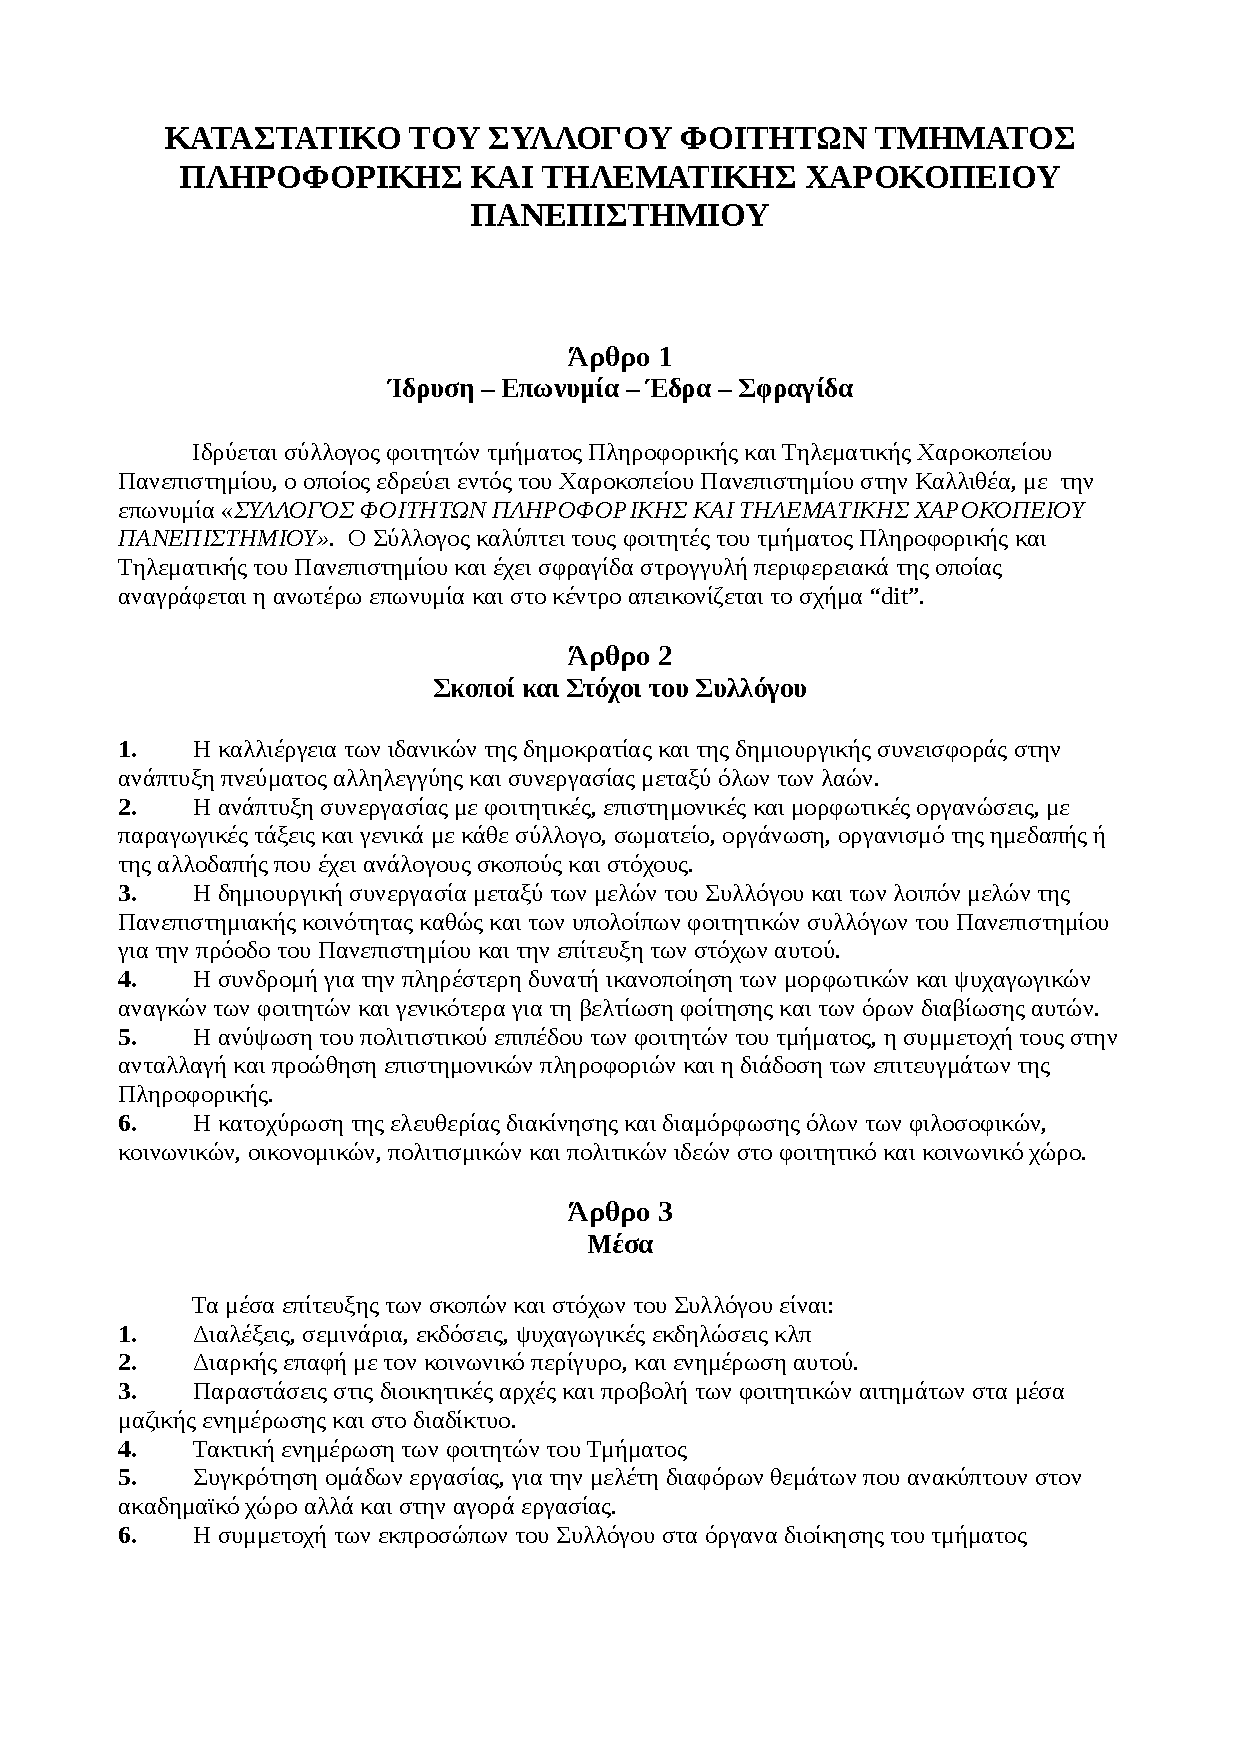
\includepdf[pages={1-8}]{katastatiko.pdf}
\end{document}
